\documentclass[table]{article}

\usepackage{hyperref}
\usepackage{graphicx}


\usepackage{fullpage}
\usepackage{tabularx}
\usepackage{amsmath}
\usepackage{amssymb}
\usepackage{amsfonts}
\usepackage{graphicx}
\usepackage{xcolor}
\usepackage{listings}
\usepackage{caption}
\usepackage{tikz}

\usepackage{array}   % for \newcolumntype macro



\newcolumntype{L}{>{$}l<{$}} % math-mode version of "l" column type
\newcolumntype{R}{>{$}r<{$}} % math-mode version of "r" column type
\newcolumntype{C}{>{$}c<{$}} % math-mode version of "c" column type


\renewcommand{\baselinestretch}{1.3}

\newcounter{questioncounter}
\setcounter{questioncounter}{1}

\newcommand{\changequestiontitle}[1]{\def\questiontitle{#1 }}
\changequestiontitle{Question}

\definecolor{codegreen}{rgb}{0,0.6,0}
\definecolor{codegray}{rgb}{0.5,0.5,0.5}
\definecolor{codelightgray}{rgb}{0.9,0.9,0.95}
\definecolor{codepurple}{rgb}{0.58,0,0.82}
\definecolor{codeyellow}{rgb}{0.51, 0.37, 0.012}
\definecolor{codemagneta}{rgb}{0.72, 0, 0.22}

\definecolor{intblue}{rgb}{0.04, 0.5, 0.84}
\definecolor{intbgblue}{rgb}{0.87, 0.92, 0.96}

\lstdefinelanguage{js} {
	keywords={typeof, new, true, false, catch, function, return, null, catch, switch, var, if, in, while, do, else, case, break},
	ndkeywords={class, export, boolean, throw, implements, import, this},
	sensitive=false,
	comment=[l]{//},
	morecomment=[s]{/*}{*/},
	morestring=[b]',
	morestring=[b]"
}

\lstset {
	aboveskip=\baselineskip,
	commentstyle=\color{codegreen},
	keywordstyle=\bfseries\color{codemagneta},
	numberstyle=\ttfamily\tiny\color{codegray},
	stringstyle=\color{codepurple},
	basicstyle=\ttfamily\footnotesize,
	breakatwhitespace=false,
	breaklines=true,
	backgroundcolor=\color{codelightgray},
	captionpos=b,
	keepspaces=true,
	numbers=left,
	xleftmargin=2em,
	numbersep=5pt,
	showspaces=false,
	showstringspaces=false,
	showtabs=false,
}
\newcommand{\N}{\mathbb{N}}

\newcommand{\question}[1]{
	\hfill \break\noindent\textbf{\color{intblue} \questiontitle  \thequestioncounter.} #1 \\ \stepcounter{questioncounter}
}




\usepackage{xepersian}
\settextfont{XB Yas}

\def\Vrulefill{
	{
		\noindent 
		\tikz\draw[intblue,fill=intblue] (0,0) circle (.5ex); 
		\color{intblue}
		\leavevmode%
		\hskip-.43in%
		\leaders%
		\vtop{\hsize=.0025in\vskip-.04in.}%
		\hfill%
		\hskip.2in%
		\tikz\draw[intblue,fill=intblue] (0,0) circle (.5ex);
	}	
}



\newcommand{\nintro}[5]{		
	\begin{center}
		\large
		
\includegraphics[scale=.3]{\basepath/beheshti_logo.jpg}\\
		#4\\\vspace{0.5cm}
	\end{center}
	\begin{center}
		\large
		\color{intblue}
		\arrayrulecolor{intblue}
		\rowcolors{1}{white}{intbgblue}
		\begin{tabularx}{\textwidth} { 
				| >{\centering\arraybackslash}X 
				| >{\centering\arraybackslash}X | }
			\hline
			\textbf{نام و نام خانوادگی} & \textbf{شماره‌ی دانشجویی} \\
			\hline
			#1  & #2  \\
			\hline
			\textbf{نام درس} & \textbf{عنوان تمرین} \\
			\hline
			#3  & #5  \\
			\hline
		\end{tabularx}
	\end{center}
	\vspace{.5cm}
	\Vrulefill \\
	\arrayrulecolor{black}
}

\def\lstlistingname{کد}% Listing -> Algorithm
\renewcommand{\lstlistlistingname}{List of \lstlistingname s}% List of Listings -> List of Algorithms
\lstdefinestyle{persian}{
	captiondirection=RTL,
	numberstyle=\tiny\lr
}

\lstset{
	style=persian,
}


\usepackage{multirow}
\begin{document}
	%\nintro{علیرضا‌ افروزی}{99222011}{پروژه‌ی پایانی نرم‌افزار ریاضی ۲}{1400-1401}{سری ۳}
	\begin{center}
		\large
		
\includegraphics[scale=.3]{./beheshti_logo.jpg}\\
		$2022$\\\vspace{0.5cm}
	\end{center}
	\begin{center}
		\large
		\color{intblue}
		\arrayrulecolor{intblue}
		\rowcolors{1}{white}{intbgblue}
		\begin{tabularx}{\textwidth} { 
				| >{\centering\arraybackslash}X 
				| >{\centering\arraybackslash}X | }
			\hline
			\textbf{نویسندگان} & \textbf{عنوان} \\
			\hline
			علیرضا افروزی، محمد کربلایی شعبانی، \hspace{2cm}محمدحسین میرقادری  & بررسی تحلیلی دیتاست مربوط به شهر نیویورک در سال ۲۰۰۹  \\
			\hline
			
		\end{tabularx}
	\end{center}
	%\vspace{.5cm}
	\Vrulefill \\
	\arrayrulecolor{blue}
	
	\section{چکیده}
	قصد داریم بر روی یک دیتاست از سال 2019 در مورد Airbnb در نیویورک فرضیاتی مطرح کنیم و به مطالعه آنها بپردازیم. به بررسی تاثیر و رابطه طول جغرافیایی بر قیمت اجاره ها یا بررسی تفاوت قیمتی انواع مسکن های اجاره ای می پردازیم.
	
	\section*{کلمات کلیدی}
	Airbnb
	،
	 اجاره، قیمت خانه، نیویورک، طول جغرافیایی.
	\section{مقدمه}
	دیتاست موجود مربوط به تمامی قراداد های اجاره مسکن در سال 2019 هست که توسط پلتفرم Airbnb در شهر نیویورک صورت گرفته است. هر قرارداد شامل اطلاعاتی در مورد اسم مسکن، اسم میزبان، محله ای که مسکن در آن واقع شده است و طول و عرض جغرافیایی مسکن و ... است. در این مورد فرضیاتی مطرح می‌شود که ما در نظر داریم که آن‌ها را بررسی کنیم:
	
	\begin{enumerate}
		\item به طور میانگین قیمت اجاره‌ی هر نوع خانه‌ای در محله‌ی منهتن از بقیه محلات بیشتر است
		
		\item وجود دارد محله ای ک قیمت اجاره‌ی \lr{private room} ش بیشتر از \lr{entire room} در محله های دیگر باشد
		
		\item اول دسته بندی کنیم طول و عرض جغرافیایی رو بعدش برسی کنیم این ادعا رو که بازه ای که بیشترین خونه درون هستند ارزون ترین بازه هم هست.
		
		\item دلیل تراکم بالای اجاره ها در این بازه 
		$[-74, -73.9]$ 
		طول جغرافیایی، قیمت ارزان تر آن به نسبت دیگر مناطق بوده است
	\end{enumerate}
	
	\noindent  این مسائل می‌توانند از چندین جنبه حائز اهمیت باشند که مهمترین آن‌ها عبارتند از:
	\begin{itemize}
		\item شناسایی خانه مناسب جهت اجاره برای استفاده با در نظر گرفتن نیاز ها و شرایط.
		
		\item نرمالیزه کردن قیمت بر اساس دیگر پارامتر‌ها و شرایط.
		
		\item بررسی پارامتر های تاثیر گذار در قیمت و کیفیت خانه های اجرایی.
		
	\end{itemize}

	\section{روش}
	\subsection{بررسی فرضیه‌ی اول}
	پس از شناسایی داده‌ها متوجه می‌شویم که در این داده‌ها، شهر نیویورک به ۵ گروه محلات تقسیم می‌شوند و در فرضیه‌ی اول ما به بررسی این می‌پردازیم که نشان دهیم به طور میانگین، اجاره‌ی گروه محلات \lr{Manhattan} از سایر گروه‌ها بیشتر است. 
	
	ابتدا ستون‌های موردنیازمان را انتخاب کرده و سایز ستون ها را از آن حذف می‌کنیم. پس از انجام این عملیات و زدن دستور 
	\verb*|data.head()|
	 خروجی زیر را خواهیم داشت:
	 
	 \begin{LTR}
	 	\begin{table}[!h]
	 		\centering
	 		\begin{tabular}{|C|C|c|c|C|C|C|}
	 			\hline
	 			& \text{id} &	neighbourhood\_group &	neighbourhood &	\text{latitude} &	\text{longitude} &	\text{price} \\ \hline
	 			0 &	2539 &	Brooklyn &	Kensington &	40.64749 &	-73.97237 &	149 \\
	 			1 &	2595 &	Manhattan &	Midtown &	40.75362 &	-73.98377 &	225 \\
	 			2 &	3647 &	Manhattan &	Harlem &	40.80902 &	-73.94190 &	150 \\
	 			3 &	3831 &	Brooklyn &	Clinton Hill &	40.68514 &	-73.95976 &	89 \\
	 			4 &	5022 &	Manhattan &	East Harlem &	40.79851 &	-73.94399 &	80 \\ \hline
	 		\end{tabular}
 		\caption{}
	 	\end{table}
	 \end{LTR}
	
	برای این که بدانیم فرضیه‌مان تا چه حد معتیر است، یک نمودار دوبعدی \lr{scatter} می‌کشیم. نقاط این نمودار با طول شناسه \lr{id} و عرض \lr{price} هستند. نکته‌ای که این نمودار دارد این است که نقاطی که مربوط به خانه‌های گروه محلات \lr{Manhattan} است به رنگ قرمز و دیگر نقاط به رنگ ابی نشان داده شده است.
	\begin{figure}[h!]
		\centering
		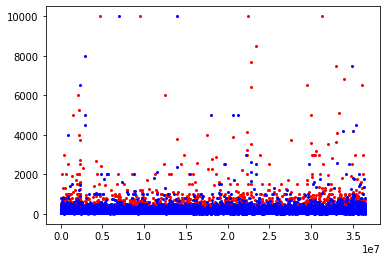
\includegraphics[scale=.6]{./graph1.png}
		\caption{}
	\end{figure}

	با در نظر گرفتن این شکل می‌توان نظارت کرد که نقاط قرمز و آبی، تقاوت چندانی با یکدیگر ندارند. یعنی نمی‌توان گفت که قیمت اجاره خانه ها در گروه \lr{Manhattan} تفاوت زیادی با دیگر گروه ها دارد. پس برای این که فرضیه‌ی خودمان را به اثبات برسانیم، نیاز داریم که یک میانگین گیری ساده روی گروه‌ها و قیمت خانه‌های مربوطه انجام دهیم. برای این کار از کد زیر استفاده می‌کنیم.
	\begin{LTR}
		\lstinputlisting[language=python]{./code1.py}
	\end{LTR}
	همینطور که کامنت شده است، خروجی این کد همان فرض ماست. در این کد متغیر
	\verb*|data|
	در واقع دیتافریم داده‌های ماست.
	برای بررسی بیشتر نمونه‌ی همین کد را روی محله‌ها به جای گروه‌های محلات اجرا می‌کنیم. پس از این اجرا، خروجی محله‌ی \lr{Fort Wadsworth} است. مانند شکل ۱، نموداری برای این محله می‌کشیم اما این بار هم بدون خانه‌های سایر محلات و هم با خانه‌های سایر محلات می‌کشیم.
	\begin{figure}[h!]
		\centering
		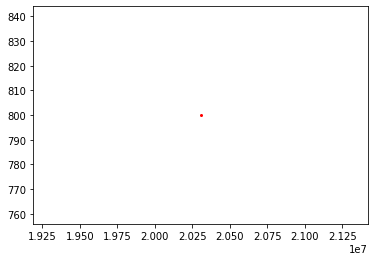
\includegraphics[scale=.5]{./graph2.png}
		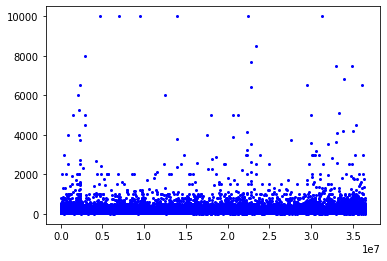
\includegraphics[scale=.5]{./graph3.png}
		\caption{}
	\end{figure}
	نمودار سمت راست، تنها شامل یک نقطه است و نشان دهنده‌ی خانه‌ای است که در محله‌ی \lr{Fort Wadsworth}  قرار دارد. یعنی تنها‌ خانه‌ای که در این محله‌ قرار دارد، به طور کلی از میانگین قیمت سایر محلات، قیمت بیشتری دارد.
	
	یک راه دیگر برای بررسی میانگین قیمت محلات، استفاده از دو ویژگی طول و عرض جغرافیایی است که با Latitude و Longitude قابل دسترسی هستند. می‌توانیم یک نمودار دوبعدی Scatter رسم کنیم که طول و عرض آن همان طول و عرض جغرافیایی باشتذ و علاوه بر آن فیمت ها را با استفاده از یک نگاشت رنگی نمایش دهیم. به صورتی که نقاطی که رنگ سرد تری دارند، کم قیمت تر و نقاطی که رنگ گرم‌تری دارند، قیمت بیشتری دارند. نمودار مربوطه به شکل زیر است:
	\begin{figure}[h!]
		\centering
		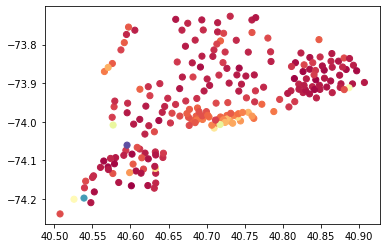
\includegraphics[scale=.5]{./graph4.png}
		\caption{}
	\end{figure}

	برای این‌که به درک بهتری از بررسی ای که می‌خواهیم کنیم برسیم، کافی است، با استفاده از نگاشت رنگی یکسانی‌، خانه هایی که در گروه Manhattan قرار دارند را به صورت جدا نمایان کنیم.
	
	\begin{figure}[h!]
		\centering
		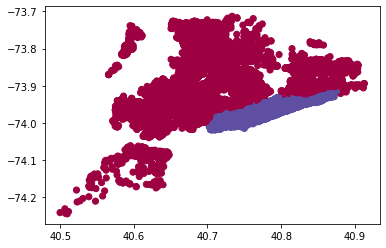
\includegraphics[scale=.5]{./graph5.png}
		\caption{}
	\end{figure}
	
	با مقایسه این دو نمودار مشخص است که خانه‌های گروه Manhattan خانه‌های به نسبت گران‌قیمت تری برای اجاره نسیت به مناطق دیگر هستند، اما این تفاوت قیمت خیلی نیست.
	
	\subsection{بررسی فرضیه‌ی دوم}
	در این فرض بررسی می کنیم که درسترس بودن یک اتاق در طول سال به چه عواملی بستگی دارد. فرض ما این است که دردسترس بودن یک نوع اتاق با تعداد اتاق های موجود  از آن نوع رابطه مستقیم و با قیمت آن نوع اتاق رابطه عکس دارد.
	
	برای بررسی عامل اول یعنی تاثیر تعداد اتاق های موجود در هر محله بر دردسترس بودن آن نوع اتاق در طول سال نمودار میله ای زیر را ترسیم می کنیم.
	\begin{figure}[h!]
		\centering
		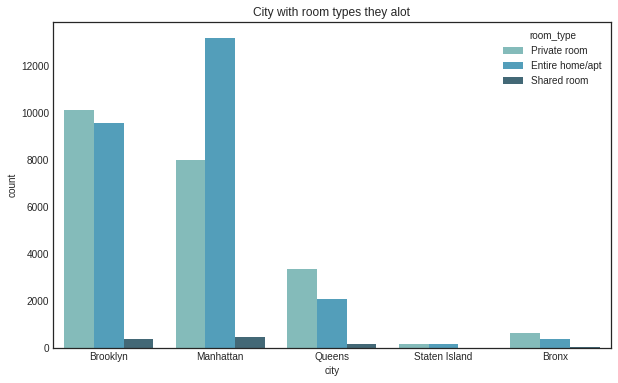
\includegraphics[scale=.5]{./graph6.png}
		\caption{}
	\end{figure}

با توجه به نمودار بالا واضح است که در تمام محله های مورد بررسی اتاق های اشتراکی (\lr{shared room}) کمترین تعداد اتاق را در مقایسه با دو نوع دیگر در اختیار دارند. در نمودار زیر به بررسی عامل دوم یعنی قیمت انواع اتاق ها می پردازیم.

	\begin{figure}[h!]
		\centering
		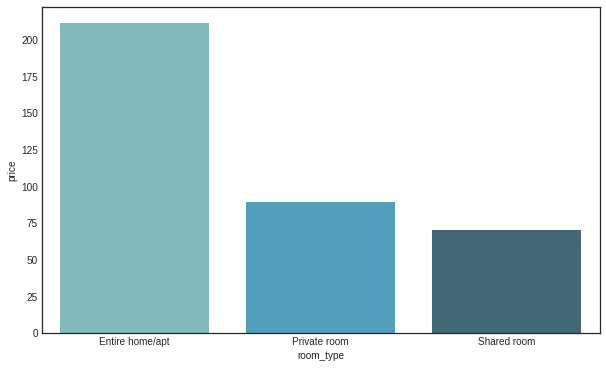
\includegraphics[scale=.5]{./graph7.png}
		\caption{}
	\end{figure}
\newpage

	همانطور که در نمودار بالا واضح است
	\begin{enumerate}
		\item 
		قیمت کل خانه بیشتر از سایر انواع است.
		\item 
		اتاق اشتراکی ارزان‌ترین است.
	\end{enumerate}

	\noindent در این مرحله برای مشخص شدن درستی یا نادرستی فرض مان دسترسی انواع اتاق ها در طول سال را در دیتاست خود بررسی می کنیم. 
	\begin{figure}[h!]
		\centering
		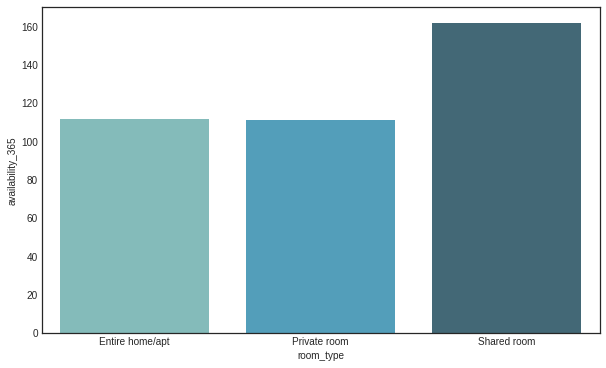
\includegraphics[scale=.5]{./graph11.png}
		\caption{}
	\end{figure}

	همانطور که در نمودار میله ای بالا مشخص است اتاق های اشتراکی در طول سال از سایر اتاق ها بیشتر در دسترس هستند. 
	\subsection{بررسی فرضیه‌ی سوم}
	فرض این است که بازه طول جغرافیایی که دارای بیشترین تعداد خانه اجاره شده است، میانگین قیمتی پایین تری نسبت به میانگین قیمتی کل خانه های اجاره شده دارد. به منظور تشخیص بازه با بیشترین تعداد خانه اجاره شده، نموندار هیستوگرام مربوط به طول جغرافیایی را میکشیم.
	\begin{figure}[h!]
		\centering
		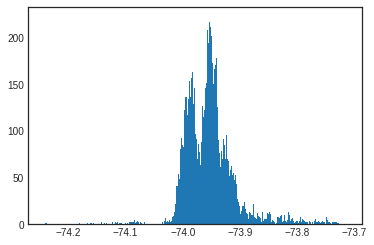
\includegraphics[scale=.6]{./graph9.png}
		\caption{}
	\end{figure}

	مشاهده میشود که بیشترین تعداد خانه اجاره داده شده در بازه طول جغرافیایی 
	$-73.9$
	تا 
	$-74$
	قرار دارند. یک دیتاست جدید میسازیم که فقط اطلاعات قرارداد هایی را داشته باشد که طول جغرافیایی آنها در بازه مذکور قرار دارد. حال نمودار هیستوگرام مربوط به سول جغرافیایی را برای داده‌های جدید رسم می‌کنیم.
	
	\begin{figure}[h!]
		\centering
		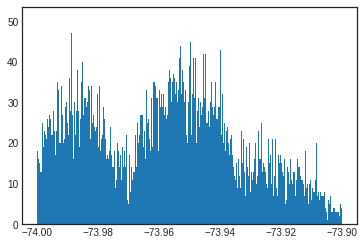
\includegraphics[scale=.6]{./graph10.png}
		\caption{}
	\end{figure}
	
	نمودار هسیتوگرام دیتاست فیلتر شده را ترسیم میکنیم مشاهده میشود که همه داده ها به درستی در بازه تعیین شده قراردارند. مقدار میانگین قیمت کل قرارداد ها و مقدار میانگین قرارداد هایی که طول جغرافیایی مطلوب را دارند به طور جداگانه حساب میکنیم. 
	
	\begin{LTR}
		\lstinputlisting[language=python]{./code2.py}
	\end{LTR}
	
	\subsection{بررسی فرضیه‌ی چهارم}
	فرضیه این است که دلیل تراکم بالای اجاره ها در این بازه طول جغرافیایی، قیمت ارزان تر آن به نسبت دیگر مناطق بوده است. دو دیتاست از به طور جداگانه از قرارداد های با طول جغرافیایی بیشتر از کران بالای بازه قبلی و از قرارداد های با طول جغرافیایی کمتر از کران پایین بازه قبلی میسازیم. حال مقدار میانگین قیمت قرارداد ها در این دو بازه را محاسبه میکنیم.
	
	\begin{LTR}
		\lstinputlisting[language=python]{./code3.py}
	\end{LTR}
	
	\section{نتیجه‌گیری}
	\subsection{نتیجه‌ی فرضیه‌ی اول}
	فرض این که قیمت‌های گروه محلات Manhattan بسیار بالا تر از قیمت گروه‌های دیگر است، اشتباه است اما می‌توان گفت در میانگین این فرض درست است. با گرفتن یک میانگین گروهی ساده روی ستون قیمت این نتیجه را میتوان گرفت. در حالت کلی گروه محلات Manhattan از محلات گران است، اما قیمت‌های این مناطق خیلی دور از قیمت های محلات دیگر نیست.
	\subsection{نتیجه‌ی فرضیه‌ی دوم}
	همانطور که در نمودار های بالا مشاهده کردیم برخلاف فرض، در دسترس بودن یک نوع اتاق به تنهایی وابسته به قیمت و تعداد اتاق موجود نیست. برای نمونه علی رغم اینکه اتاق های اشتراکی کمترین تعداد اتاق را دارا هستند و همچنین کمترین قیمت را در مقایسه با سایر اتاق ها دارند اما در طول سال بیشتر از سایر اتاق ها در دسترس هستند. این نشان دهنده عدم رغبت مسافران به اجاره اتاق های اشتراکی می باشد. به طور کلی می توان گفت که حریم خصوصی ، امکانات رفاهی و مدیریت زمان و فضای سکونت از عوامل و متغیر های اصلی برای انتخاب و اجاره یک اتاق می باشد.
	
	نمودار زیر به وضوح صحت نتیجه گیری بالا را نشان می دهد
	
	\begin{figure}[h!]
		\centering
		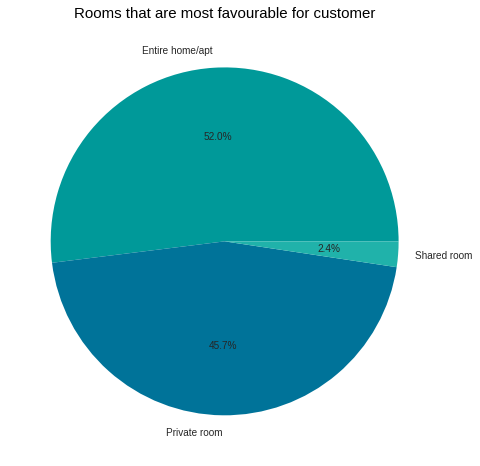
\includegraphics[scale=.5]{./graph8.png}
		\caption{}
	\end{figure}

\newpage
	\subsection{نتیجه‌ی فرضیه‌ی سوم}
	\begin{LTR}
		\lstinputlisting[language=python]{./code2.py}
	\end{LTR}
	
	مشاهده میشود که فرضیه ما درست بوده است و میانگین قیمت در این بازه از میانگین قیمت کل قرارداد ها کمی کمتر است. حال میتوان ادعا کرد که دلیل تراکم بالای اجاره ها در این بازه طول جغرافیایی، قیمت ارزان تر آن به نسبت دیگر مناطق بوده است.
	\subsection{نتیجه‌ی فرضیه‌ی چهارم}
	با توجه به اینکه میانگین قیمت در بازه طول جغرافیایی بزرگتر از کران بالای بازه مطلوب ما، کمتر است از میانگین قیمت در بازه مطلوب، ادعای ما رد میشود چرا که اگر قیمت پایین دلیل تراکم بالای قرارداد ها در آن منطقه بود باید تراکم قرارداد ها در این بازه که میانگین قیمت کمتری دارد بیشتر  می‌بود.
	
	\section{منبع}
	\begin{itemize}
		\item \url{https://www.kaggle.com/dgomonov/new-york-city-airbnb-open-data}
	\end{itemize}
\end{document}